%%This is a very basic article template.
%%There is just one section and two subsections.
\documentclass{article}

\usepackage{a4wide}
\usepackage{amsmath}
\usepackage{float}
\usepackage{listings}
\usepackage{graphicx}
\usepackage{epstopdf}

\lstset{ %
breaklines=true,
language=R
}

\begin{document}

\title{Probability and Statistics for Data Analysis\\Assignment 2}
\author{Charalampos Kaidos}

\maketitle

\section*{Exercise 8}

In the spreadsheets named W, X, Y and Z of the file Assignment\_2\_data.xlsx
(available on e-class assignments site) there are data sets from various random
variables. Each student will take one column of data from each of these four
spreadsheets (columns assignment to students will be done in class). For each of
these four univariate samples, that you will be assigned, you need to:

First we read the data. I used the xlsx library to read the excel file, then
picked each sheet and stored it in CSV format to allow easier access and storage
to CVS. I use these csvs to load the data. My column is 5.

\begin{lstlisting}
#First column is the row names stored in csv
my_column <- 5 + 1 

W <- read.csv(file = "w.csv")[[my_column]]
X <- read.csv(file = "x.csv")[[my_column]]
Y <- read.csv(file = "y.csv")[[my_column]]
Z <- read.csv(file = "z.csv")[[my_column]]
\end{lstlisting}

\begin{enumerate}
  \item Provide various forms of graphical representation of the data.
  First we are going to plot the data we have using simple scatterplots. We want
  to get a feeling what we are dealing with:
  \begin{lstlisting}
par(mfrow = c(2,2))
  
plot(sort(W), main = "W", ylab = "W")
plot(sort(X), main = "X", ylab = "X")
plot(sort(Y), main = "Y", ylab = "Y")
plot(sort(Z), main = "Z", ylab = "Z")
  \end{lstlisting}
  
  As we can see on figure~\ref{fig:scatterplots} (p~\pageref{fig:scatterplots})
  The data in W and X are discrete while the data in Z are continuous. The data
  in Y seem to be zero all but a few values. We will investigate Y further.
  
  \begin{figure}[H]
  \centering
  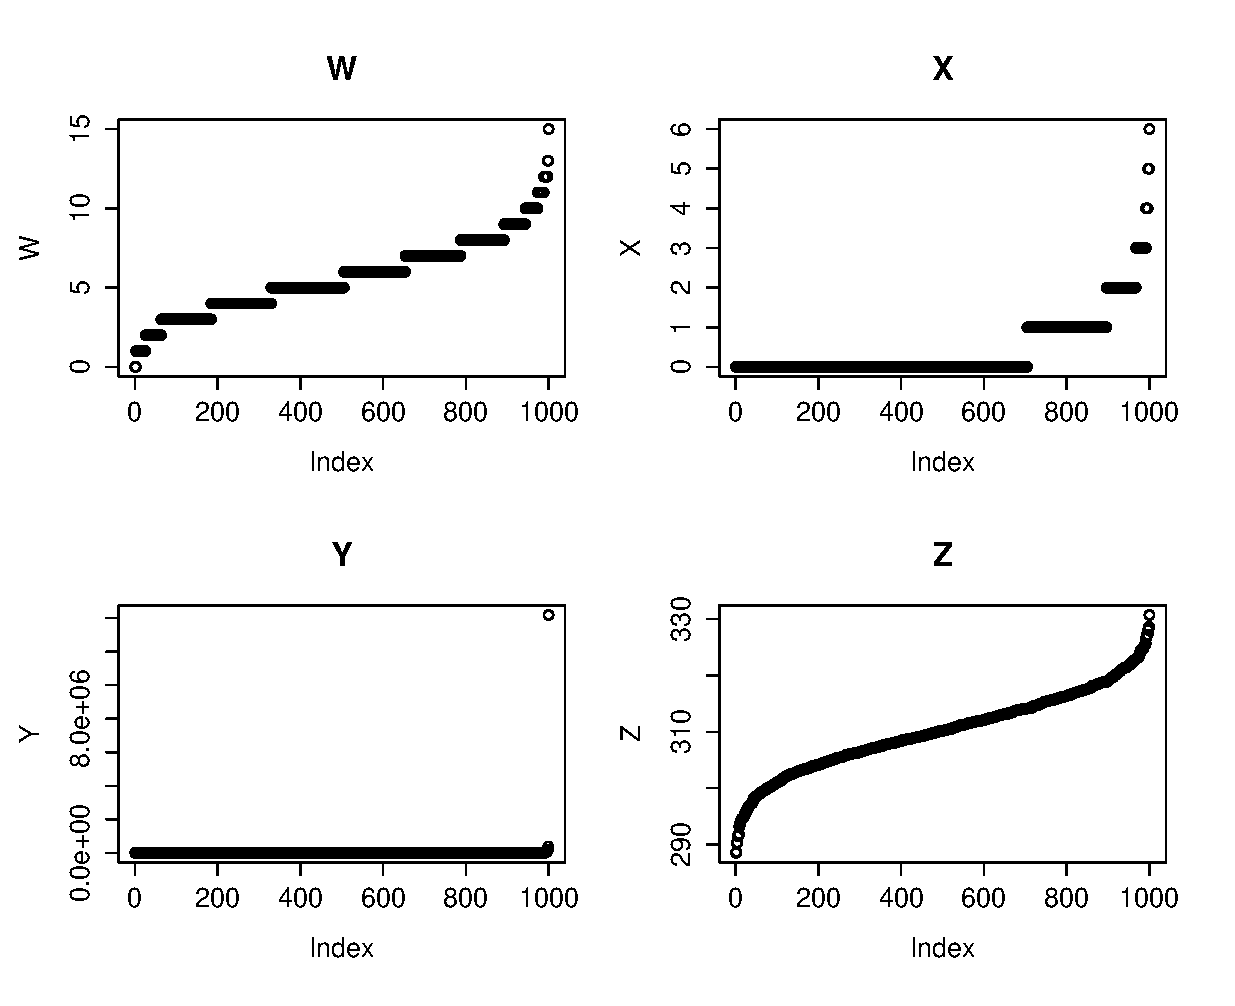
\includegraphics[scale=0.6]{scatterplots.eps}
  \caption{Scatter plots}
  \label{fig:scatterplots}
  \end{figure}
  
  We attempt to plot the data in Y without the last, without the 100 last and
  whithout the 500 last samples (figure~\ref{fig:scattery},
  p.~\pageref{fig:scattery})
  
  \begin{lstlisting}
par(mfrow = c(1,3))

plot(sort(Y)[0:999], main = "Y without highest sample", ylab = "Y")
plot(sort(Y)[0:900], main = "Y without highest 100 samples", ylab = "Y")
plot(sort(Y)[0:500], main = "Y without highest 500 samples", ylab = "Y")
  \end{lstlisting}
  
  We can see that the values in Y are increasing in an exponential range. This
  will be usefull later.
  
  \begin{figure}[H]
  \centering
  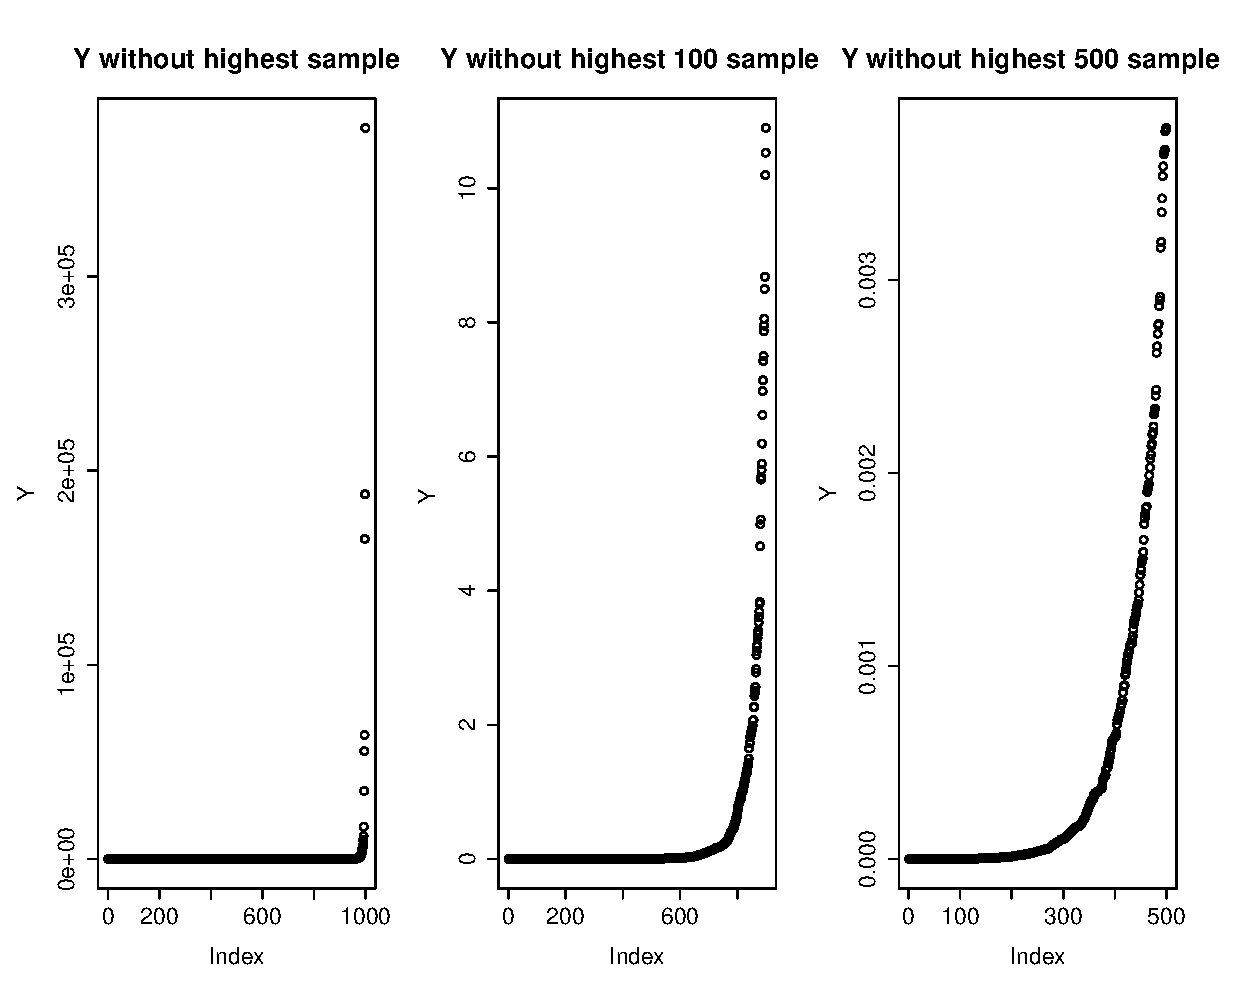
\includegraphics[scale=0.6]{scattery.eps}
  \caption{Y scatter plots}
  \label{fig:scattery}
  \end{figure}
  
  Next we will plot histograms from these data to get a hint of the
  distributions that may have generated them (figure~\ref{fig:histograms},
  p.~\pageref{fig:histograms})
  
  \begin{lstlisting}
par(mfrow = c(2,2))

hist(W, col=terrain.colors(15))
hist(X, col=terrain.colors(15), breaks=c(0:8), right = FALSE, include.lowest = FALSE)
hist(Y, col=terrain.colors(15))
hist(Z, col=terrain.colors(15))
  \end{lstlisting}
  
  \begin{figure}[H]
  \centering
  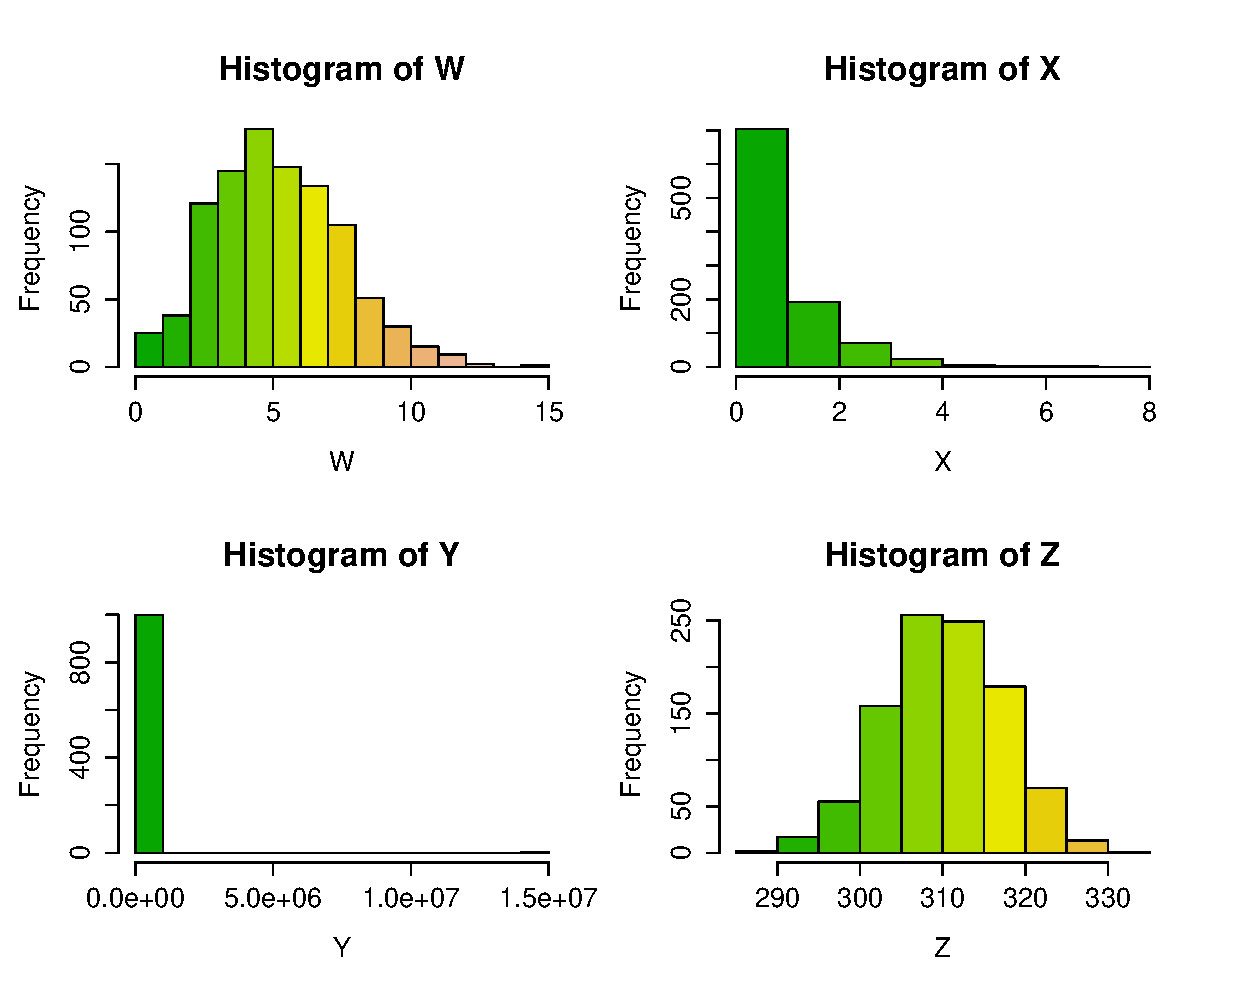
\includegraphics[scale=0.6]{histograms.eps}
  \caption{Histograms}
  \label{fig:histograms}
  \end{figure}
  
  Finally the boxplots will show the quantiles and outliers of the data
  (figure~\ref{fig:boxplots}, p.~\pageref{fig:boxplots})
  
  \begin{lstlisting}
par(mfrow = c(2,2))

boxplot(W, col=terrain.colors(15), ylab = "W")
boxplot(X, col=terrain.colors(15), ylab = "X")
boxplot(Y, col=terrain.colors(15), ylab = "Y")
boxplot(Z, col=terrain.colors(15), ylab = "Z")
  \end{lstlisting}
  
  \begin{figure}[H]
  \centering
  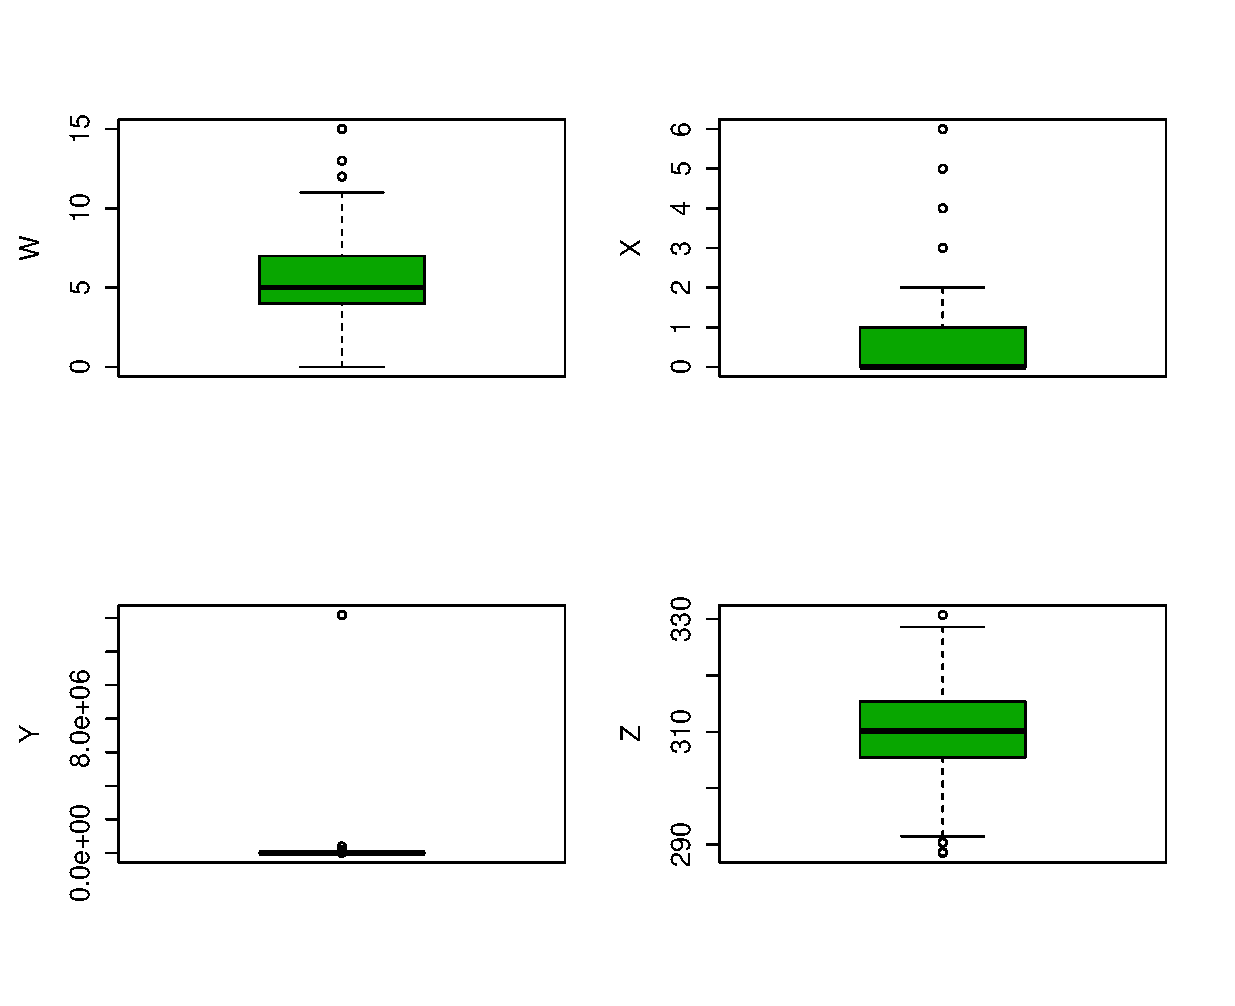
\includegraphics[scale=0.6]{boxplots.eps}
  \caption{Box plots}
  \label{fig:boxplots}
  \end{figure}

  \item Describe  the  type  of data  along  with  various  descriptive 
  statistics  that  could provide insight on which is the generating random variable.
  
  For each data column we will find the data type, the minimum and maximum
  values, the first, second and third quantiles, the mean, the variance and
  standard deviation, the skewness and the kyrtosis.
  
  \begin{lstlisting}
> class(W)
[1] "integer"
> head(W)
[1] 5 0 5 5 4 7
> summary(W)
   Min. 1st Qu.  Median    Mean 3rd Qu.    Max. 
  0.000   4.000   5.000   5.661   7.000  15.000 
> var(W)
[1] 5.36144
> sd(W)
[1] 2.315478
> skewness(W)
[1] 0.3750572
> kurtosis(W)
[1] 3.054172
  \end{lstlisting}
  
  The first data set W is a list of integers and we verify that by printing the
  first 6 samples. 0 is the minimum value while 15 is the maximum. The first
  quantile is at 4, the median is 5 and the third quantile is at 7. The mean is
  5.661, the variance is 5.361 and the standard deviation 2.315. The skewness is
  0.375 which means that the data are a bit right skewed. Finally the kurtosis
  is 3.054 which makes it mesokurtic.
  
  \begin{lstlisting}
> class(X)
[1] "integer"
> head(X)
[1] 0 1 1 0 0 0
> summary(X)
   Min. 1st Qu.  Median    Mean 3rd Qu.    Max. 
  0.000   0.000   0.000   0.447   1.000   6.000 
> var(X)
[1] 0.6838749
> sd(X)
[1] 0.8269673
> skewness(X)
[1] 2.326085
> kurtosis(X)
[1] 9.674228
  \end{lstlisting}
  
  The second data set X is also a list of integers printing the first 6 samples.
  The minimum is 0 and the maximum is 6. The first and second quantiles are both
  at 0 while the third is at one. The mean is 0.447, the variance 0.684 and the
  standard deviation 0.827. The skewness is 2.336 so it is stronly skewed to the
  right and leptokurtic since the kurtosis is 9.674.
  
  \begin{lstlisting}
> class(Y)
[1] "numeric"
> head(Y)
[1] 3.038756e-05 1.906351e-02 9.832293e-08 2.708900e-02 2.103855e-01 1.554413e+01
> summary(Y)
    Min.  1st Qu.   Median     Mean  3rd Qu.     Max. 
       0        0        0    15160        0 14190000 
quantile(Y)
          0%          25%          50%          75%         100% 
8.307445e-13 4.111156e-05 3.806345e-03 2.162291e-01 1.418878e+07 
> var(Y)
[1] 201506406010
> sd(Y)
[1] 448894.6
> skewness(Y)
[1] 31.52599
> kurtosis(Y)
[1] 995.8972
  \end{lstlisting}
  
  The Y data set is a list of floats. The summary doesn't give much information
  for values close to 0 so we use the quantile function. The minimum is
  $8.2*10^{-13}$ while the maximum is $1.4*10^{7}$. The first quantile is at
  $4.1*10^{-5}$, the median is $3.8*10^{-3}$ and the third quantile is
  $2.1*10^{-1}$. The mean is 15160, the variance 201506406010 and the standard
  deviation 448894.6. The sample comes from a distribution that is very skewed
  to the right with skewness 31.525 and very leptokurtic with kurtosis 995.
  
  \begin{lstlisting}
> class(Z)
[1] "numeric"
> head(Z)
[1] 318.3571 309.2381 305.4094 312.0540 313.5075 307.6789
> summary(Z)
   Min. 1st Qu.  Median    Mean 3rd Qu.    Max. 
  288.5   305.4   310.2   310.2   315.4   330.7 
> var(Z)
[1] 50.21331
> sd(Z)
[1] 7.086135
> skewness(Z)
[1] -0.08839937
> kurtosis(Z)
[1] 2.821732
  \end{lstlisting}
  
  The last data set Z is a list of floats with minimum 288.5 and maximum 330,7.
  The first quantile is at 305.4, the second is at 310.2 and the third at 315.4.
  The mean is 310.2, the variance is 50.213 and the standard deviation 7.087.
  Fianlly it is slightly skewed to the left (skewness -0.089) and slightly
  platikurtic (kurtosis 2.821).
  
  \item Based on (a) and (b) search for the random variable that fits best the
  observed data.
  
  The data from column W looks like it could be from many distributions. After
  some trial and errors and a few functions that search the parameters we have
  found a distribution we cannot reject. It is plausible that the data of W come
  from a Poisson distribution with $lambda=5.7$. The chi-squared test confirms
  the hypothesis.
  
  \begin{lstlisting}
t<-test.pois(W, 5.7)
$p.value
[1] 0.4662631

$method
[1] "Chi-squared test for given probabilities"
  \end{lstlisting}
  
  The data from the X column are discrete with high probability on 0. Poison
  seems like a good candidate but after some experimentation we find out that a
  good choice is the nagative binomial with 1 succesfull trial and probability
  0.7. The chi-squared test confirms this is a valid hypothesis:
  
  \begin{lstlisting}
> quantiles <- seq(min(X),max(X))
> distribution <-dnbinom(quant,size = 1,prob = 0.7)
> chisq.test(x = c(table(X),0), p = c(distribution, 1-sum(distribution)))

	Chi-squared test for given probabilities

data:  c(table(X), 0)
X-squared = 5.7176, df = 7, p-value = 0.5731
  \end{lstlisting}
  
  The Y data set doesn't seem to be from a known distribution. The values though
  seem to be exponential. We will try to tranform the values and see what
  happens.
  
  \begin{lstlisting}
> logY <- log(Y)
> class(logY)
[1] "numeric"
> head(logY)
[1] -10.401477  -3.959979 -16.135009  -3.608628  -1.558814   2.743683
> summary(logY)
   Min. 1st Qu.  Median    Mean 3rd Qu.    Max. 
-27.820 -10.100  -5.571  -5.715  -1.531  16.470 
> var(logY)
[1] 39.93254
> sd(logY)
[1] 6.31922
> skewness(logY)
[1] 0.008447037
> kurtosis(logY)
[1] 2.983757
  \end{lstlisting}
  
  The data above as well as the graphs in figure~\ref{fig:logy}
  (p.~\pageref{fig:logy}) show that logY resembles very much a $N(5.7,6.3)$.
  
  \begin{figure}[H]
  \centering
  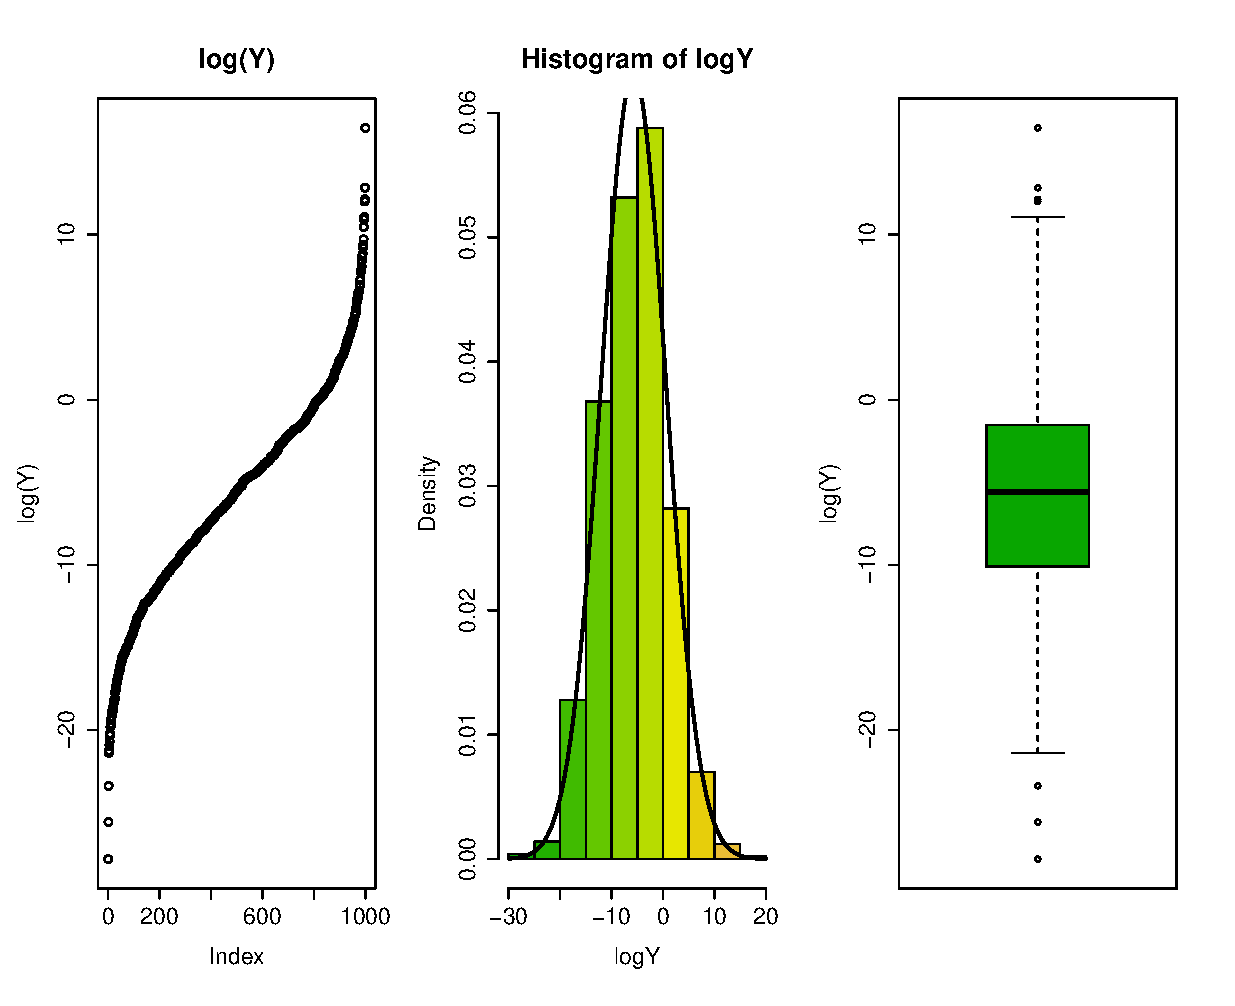
\includegraphics[scale=0.6]{logy.eps}
  \caption{log(Y)}
  \label{fig:logy}
  \end{figure}
  
  We will execute the Shapiro-Wilk normality test to see if we can reject this
  hypothesis.
  
  \begin{lstlisting}
> shapiro.test(logY)

	Shapiro-Wilk normality test

data:  logY
W = 0.99929, p-value = 0.976
  \end{lstlisting}

  Thus we cannot reject the hypothesis. We will also try the Kolmogorov-Smirnov
  test:
  
  \begin{lstlisting}
> ks.test(logY, "pnorm", mean(logY), sd(logY))

	One-sample Kolmogorov-Smirnov test

data:  logY
D = 0.023883, p-value = 0.6183
alternative hypothesis: two-sided
  \end{lstlisting}
  
  Neither this one rejects the hypothesis that logY is a normal distribution.
  Thus we can assume that Y is from a logNormal distribution. We get the same
  result when we run the Kolmogorov-Smirnov test for the logNormal:
  
  \begin{lstlisting}
> ks.test(Y, "plnorm", mean(logY), sd(logY))

	One-sample Kolmogorov-Smirnov test

data:  Y
D = 0.023883, p-value = 0.6183
alternative hypothesis: two-sided
  \end{lstlisting}
  
  For the sample Z we observe that it is almost symetrical, very lightly
  skewed, the kurtosis is close to 3. We can make the hypothesis that the data in Z
  are from a $N(310.2, 7.087)$.
  
  We see that this may be a valid hypothesis if we plot the $N(310.2, 7.087)$
  over the histogram in figure~\ref{fig:z}, p.~\pageref{fig:z}
  
  \begin{lstlisting}
hist(Z, col=terrain.colors(15), freq = F)
curve(dnorm(x, mean=mean(Z), sd=sd(Z)), add=TRUE, lwd=2)
  \end{lstlisting}
  
  \begin{figure}[H]
  \centering
  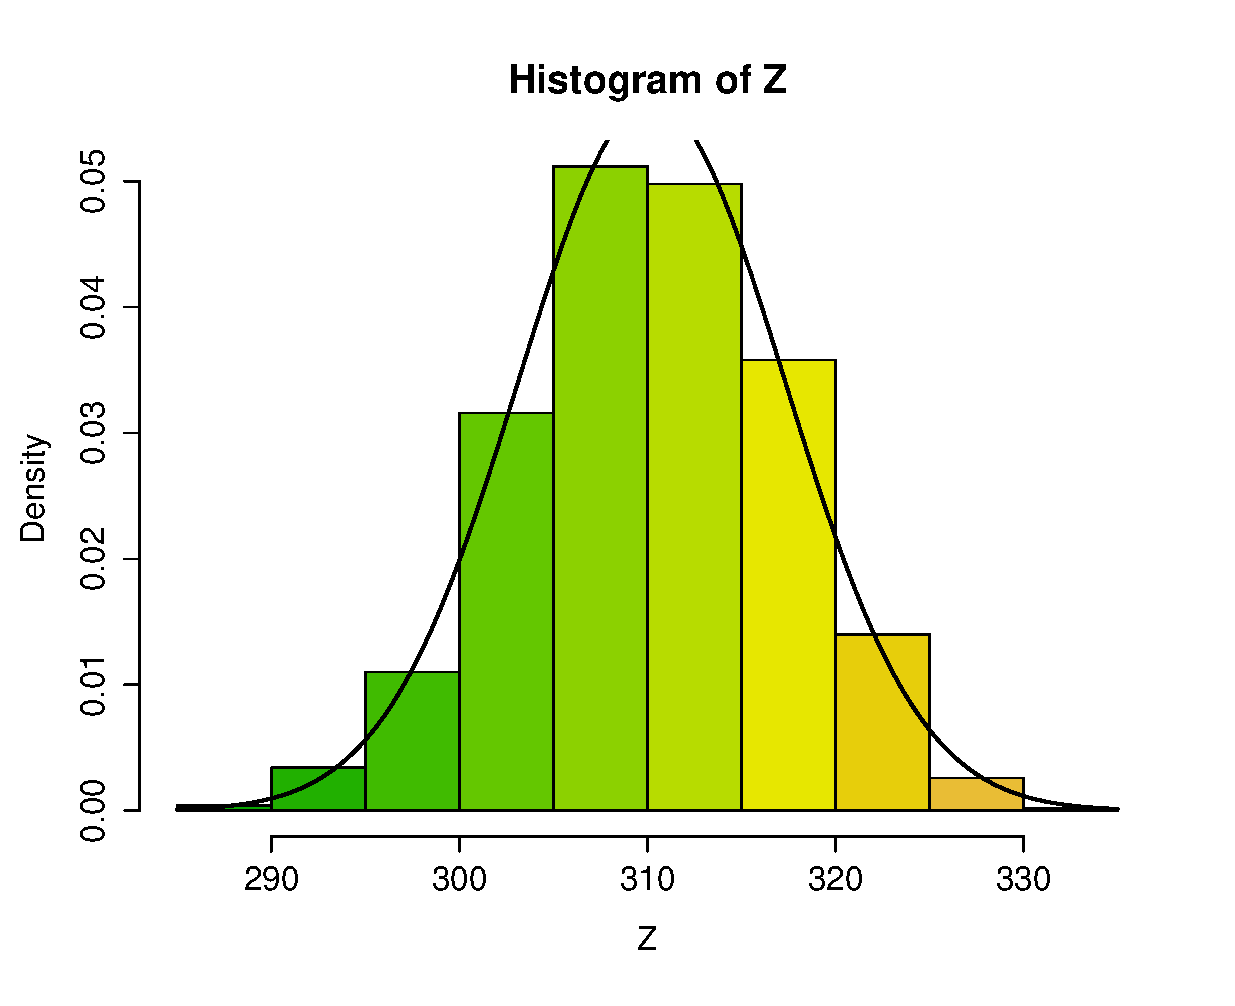
\includegraphics[scale=0.6]{z.eps}
  \caption{Z density}
  \label{fig:z}
  \end{figure}
  
  We can perform the Shapiro-Wilk normality test to check our hypothesis:
  
  \begin{lstlisting}
> shapiro.test(Z)

	Shapiro-Wilk normality test

data:  Z
W = 0.99846, p-value = 0.5307
  \end{lstlisting}
  
  From the Shapiro-Wilk test we cannot reject the hypothesis that Z is from a
  normal distribution. We will also try the Kolmogorov-Smirnov test.
  
  \begin{lstlisting}
> ks.test(Z, "pnorm", mean(Z), sd(Z))

	One-sample Kolmogorov-Smirnov test

data:  Z
D = 0.01831, p-value = 0.8908
alternative hypothesis: two-sided
  \end{lstlisting}
  
  Neither the Kolmogorov-Smirnov test rejects the hypothesis. Thus we can assume
  that Z is from a $N(310.2, 7.087)$.
  
  \item Provide point estimates of the unknown parameter(s) of the best fitted
  model.
  
\end{enumerate}

\end{document}
